%        File: main.tex
%     Created: Mon Jan 30 10:00 AM 2017 I
% Last Change: Mon Jan 30 10:00 AM 2017 I
%
\documentclass[a4paper]{article}
\usepackage[]{hyperref,graphicx}
\usepackage{csquotes}
\usepackage{xcolor}
\hypersetup{
    colorlinks,
    linkcolor={red!50!black},
    citecolor={blue!50!black},
    urlcolor={blue!80!black}
}
\DeclareGraphicsExtensions{.pdf,.png,.jpg}
\usepackage[backend=bibtex,style=numeric]{biblatex}
\addbibresource{sources.bib}
\title{State and Marriages: A Case Study}
\author{Jerin Philip}
\date{201401071}
\begin{document}
\maketitle
\tableofcontents

\section{Introduction}
One might think why it is State's business to
interfere with the marriage customs and it's
necessity to formalize or legalize and record
marriages of the people forming it. Perhaps the
Marxist theory of how family and private property
led to the formation is useful here. Marriage
being a factor in inheritance gets private
property involved, and altogether becomes State's
business.

Here, we take the case of what is today Kerala
during a period of British rule. The players were
Malabar, Travancore and Cochin, with population
predominantly Hindu - comprised of many castes and
sub castes, with a minority growing population of
Christians and Muslims. Forms of matrilineal
marriage and inheritance systems prevalent in the
area almost died out in a decade towards the end
of the Colonial rule. Other practices like
polyandry and polygamy didn't survive the colonial
period either.

Discretizing the changes to pre and post colonial
days, one perspective to look at it is how the
indigenous culture with strong matrilineal sway
got replaced with the patriarchal system more
familiar with the west. Whether the colonial State
and it's government had direct or indirect
involvements in the process is a topic of
interest. Among direct interventions, that of the
Malabar Marriage Act stands out. Also, the
colonizer's education system could also have
gradually programmed the society into the paradigm
shift.

The Malabar Marriage Commission, formed in 1891 in
response to a bill introduced by Sir C. Shankara
Nair \cite[1]{menon1894report} with the objective
of provide evidence on the customs and the
feasibility of the changes proposed by the
bill\cite[3]{menon1894report}. The operations and
report of the commission provides an ample area to
investigate how State accommodated the existing
marriage customs and how it intervened to bring
reforms, which is the primary topic in this paper.

Aside from direct interventions like an act, the
State indirectly brought about reforms and opened
the people's mind for new thinking by updated
education policies through which the content
learned by the newer generations were curated. An
literacy figures with the time - the time period
in which the acts containing reforms the Colonial
Authorities wanted were brought into effect.

\section{Sources}

The major primary source is the \emph{Report of
the Malabar Marriage Commission}. Other primary
sources include \emph{Acts and Proclamations of
Travancore}, the \emph{Malabar Manual} by William
Logan.  Several statistics are obtained from the
\emph{Census of India} data available during the
period and is referenced internally in the above
primary sources.


\section{Marriage and Inheritance Structure} 

It is important to understand the existing
structure and laws of marriage and inheritance
before examining how and why the State would want
to intervene. 
\subsection{\emph{Marumakkathayam} System}
\emph{Sambhandham} is the formal term used to
denote marriage in the context of Kerala Society.
The term \emph{Marumakkathayam} relates to property
inheritance, with all people in a household,
\emph{Tarawad} tracing their lineage back to a
female ancestress\cite[51]{menon1894report}.
The \emph{Karanavan}, senior male in the family
serves as the head of the family and manager of
the family's riches.

\blockquote[{\cite[51]{menon1894report}}]{
    Secured by the impartibility of the estate,
    refreshed by the acquisition of the junior
    members, and under the beneficent sway of the
    senior male, the \emph{Tarawad} should wax
    great and endure throughout all generations 
}

The practitioners according to the 1881 Census
Report is a minority of 30 percent in the region, but
comprising of the
aristocracy\cite[7]{menon1894report}. The below
table depicts the detailed statistics:

\begin{center}
\begin{tabular}{l r r}
    Castes & Males & Females\\
    \hline
    Kshatriyas, Nayars and the allied castes &
    233,155 & 237,174\\
    Marumakkathayam Tiyyans (North Malabar) &
    108,639 & 111,806\\
    Marumakkathayam Mukkuvans (ditto) & 2,835 &
    2805 \\
    \hline
    Total & 244,529 & 351,785\\
    \hline
\end{tabular}
\end{center}

Aside from this, there were rules that a female
from one caste or class couldn't be wed to someone
of a lower strata of the society, while for the
males, this rules didn't apply.

\subsection{People under \emph{Marumakkathayam}}
There are many perils to the above system. Many
women of the higher classes weren't able to find a
suitable groom and die in a state of celebacy
\cite[127-128]{logan1887malabar}. Only rich
households of Namboodiris were able to marry women
off at a suitable age. The population stats above
clearly indicate the females almost equal to the
male population, but males courting women in the
lower strata led to the skew. 

The families huddled together under one roof
creates a chaotic situation. ``Not a day passes,
without some fight or the other''
\cite[55]{menon1894report}, remarks a witness.
The \emph{Karanavans} and \emph{Anandravans} of
the house are always in hatred and dissension
\cite[55]{menon1894report}. Property is joint, and
treated by the \emph{Karanavan} as his own
property \cite[55]{menon1894report}. The
instability of the \emph{Tarawad} system echoes
among a lot of witnesses.

In short, there was growing discontent among those
who were subject the existing uncodified marriage
and inherit system, which caused an outcry from
the people. There was a lack of progress from the
State's point of view, due to the above problems.

\subsection{Conflicts with the State}
With ceremonial customs and degree of formality
varying with places and communities, the above
system was practised under different names closely
coupled with religion and beliefs. The above were
believed to have laid down by \emph{Parasurama}
\cite[24]{menon1894report} and not codified
uniformly. State's first problem
arose here, wherein it could not settle disputes
on property or marriages unless this was made into
a law. 

According to the witnesses examined by the Malabar
Marriage Commission, the chastity of a woman
under \emph{Marumakkathayam} system was not a big
deal, they were allowed to consort more than one
man \cite[24]{menon1894report}. Both parties are
free to announce divorce and end the union whilst
succession being through the female line which
leads to the \emph{Karanavan}'s affection for his
sister's children being more than that for his own
progeny \cite[262]{panikkar1918some}, which
British found quite unnatural.

The next problem State found with the system was
it's lack of accountability when it comes to
subsistance. Consider the following family tree.


\begin{figure}[!ht]
    \begin{center}
        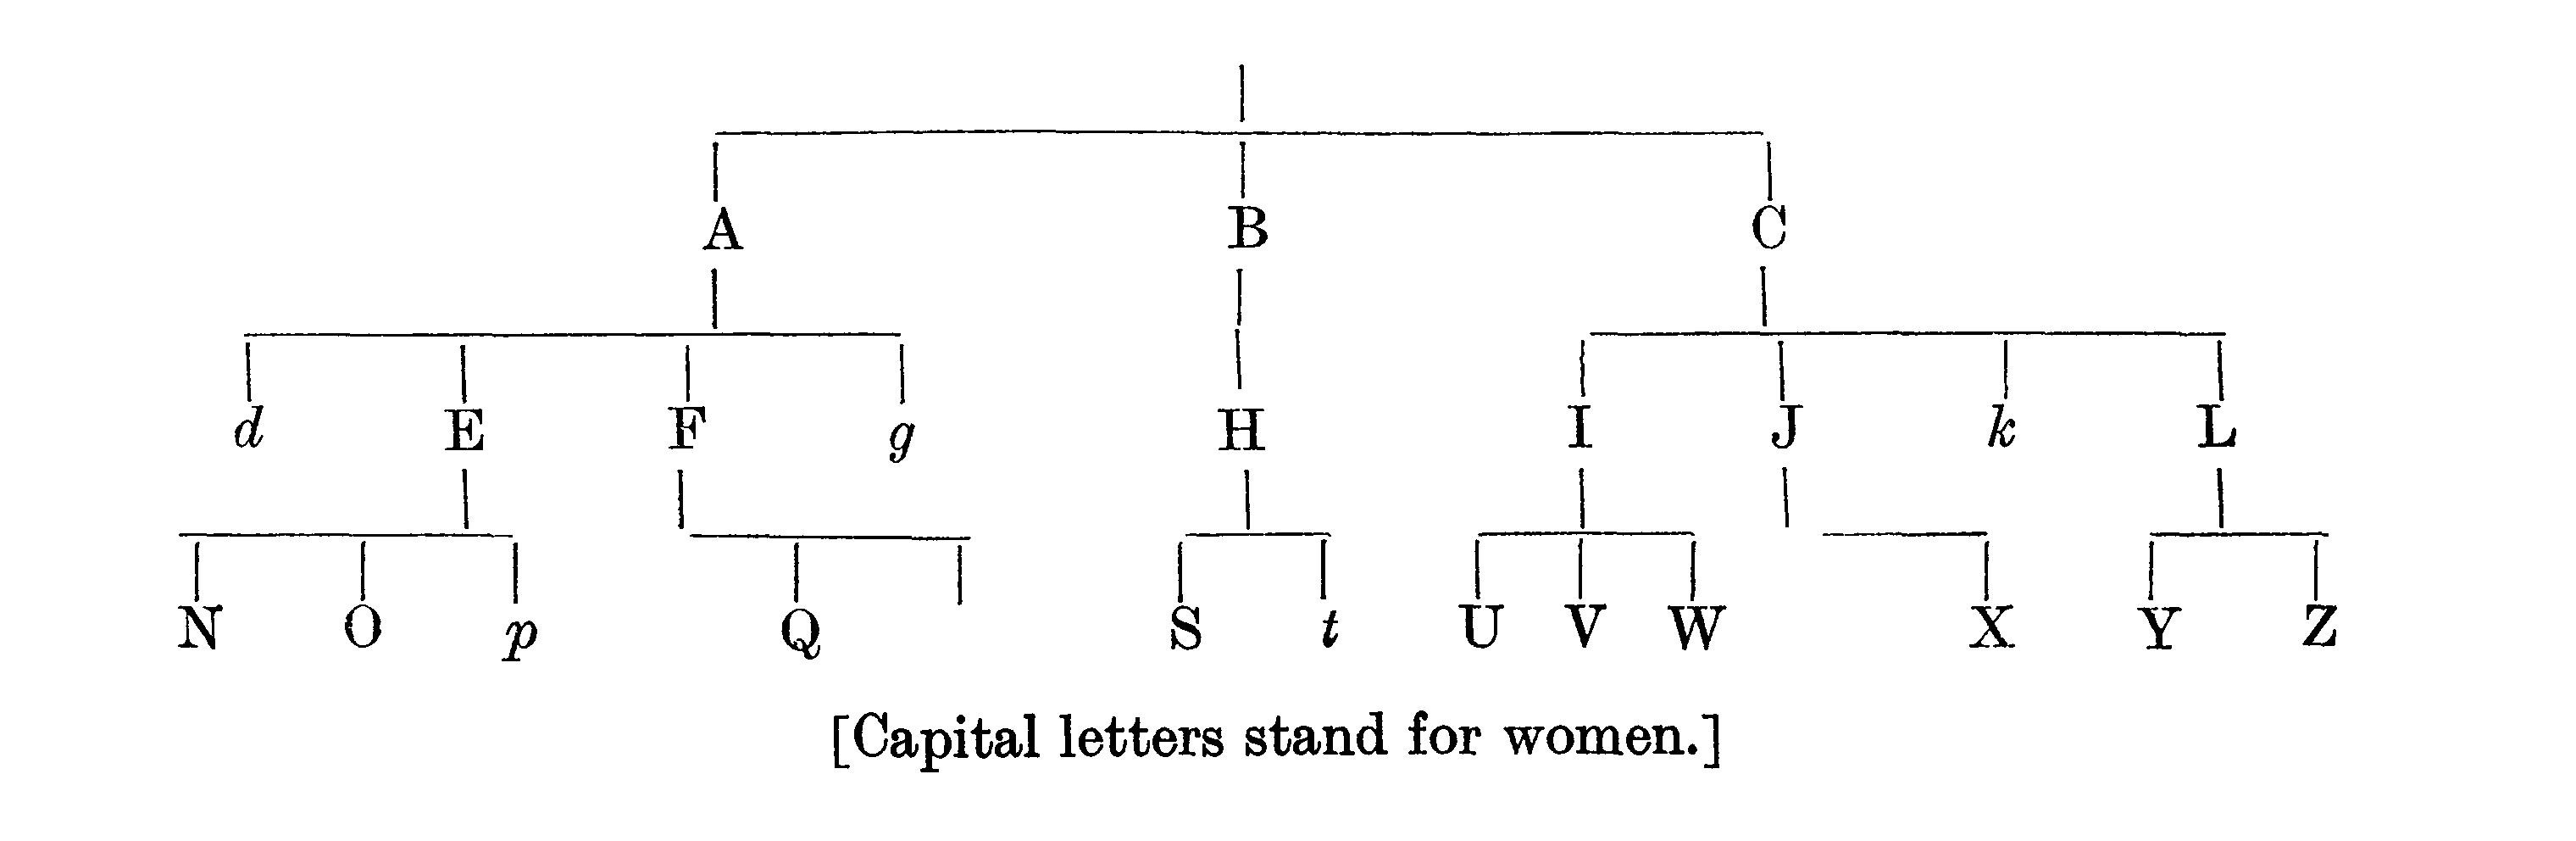
\includegraphics[width=0.8\textwidth]{marum_family_tree}
    \end{center}
    \caption{Taken from \cite[261]{panikkar1918some}}
\end{figure}

The property was being evenly distributed among
the female members of the family while the
breeding was uncontrolled, the \emph{Karanavan}
had no say, rendering uneven division of estate
few rich, and a large portion being poor and
unable to subsist which creates a problem since it
is the State's duty to bring about progress and
maintenance of laws which enable progress. ``With a
large increase in their numbers and comparative
poverty for the large body of them, the race is
fast degenerating'', writes William Logan
\cite[138]{logan1887malabar}. 

The commission set to investigate
\emph{Marumakkathayam} system concludes that it
``offends against every principle of political
economy and healthy family life'', ``sanctions
reckless propagation of the species'', ``forces
population to a point where it must be kept down
by actual want of the means of subsistence''.

The lack of laws enable a Nayar husband to
``savagely avenge''\cite[63]{menon1894report}
neglect of the marriage tie, where upon the
offender is punished immediately even by death.
This questions the State's monopoly over violence,
which could not have been tolerated.


\subsection{Decline of the \emph{Marumakkathayam}}
1870s saw a raise in voices against the system,
and the outcry led to the The Malabar Marriage
Act. This was however a failed attempt, but was
brought to the colonial State and the people's
attention. The Namboothiris collectively decided
to stop following the system sometime near 1920,
and was formalized through the 1933 Madras
Namboothiri Act. A Madras Marumakkathayam Act was
passed the same year which changed property
inhertance laws drastically, which gave way to the
decline of the \emph{Marumakkathayam} system.

Remnants of the system today exist in practices.
In few communities, the children still take the
surname of their mother, even though inheritance
and authority is passed on through the father. The
early practitioners have completely shifted from a
matrilineal to patrilineal system. Polyandry has
been completely eliminated, with the newer
generations completely unaware that it existed. 

\section{State Interventions}
In the previous section, we set the premises by
describing \emph{Marumakkathayam} system and areas
where the State found itself in conflict with the
existing practices. In this section, we take a
look at how the State, under British rule
went about to resolve the conflicts and bring the
order it desired.

\subsection{Malabar Marriage Commission}
The Malabar Marriage Bill, which was later passed
accepting suggestion of from the Commission is an
example of State directly intervening in the
marriage affairs of the state.  

The challenges faced by Commission is evident at
several places in its report
\cite{menon1894report}. One major concern is to
make sure the law passed covers all communities
and enables High Courts of the judicial polity of
State to take decision in case of disputes.
Another challenge is getting the new law to be
accepted by the masses which it rules, and how
quickly the acceptance can happen. 

Commission's recommendation included two
proposals:

\blockquote[{\cite[65]{menon1894report}}]{
    \begin{itemize}
        \item One proposal (favoured by our
            President) is to frame a marriage-law
            such as the whole body of
            \emph{Marumakkathayam} people may at
            once be able to welcome and adopt, and
            thus to engraft the institution of
            marriage upon \emph{Marumakkathayam} in such
            a form that the two may flourish
            together.  Such a law amongst other
            things must prohibit marriages
            offending against existing rules of
            caste, must provide a ready means of
            divorce without resort to Court, and
            must recognize the Marumakkathayam Law
            of Succession as meriting countenance
            and perpetuation.  
        \item The other alternative is to recommend
            a marriage-law,—such as we are sure
            that an English Government can and
            will grant,—not widely diverging in
            principle from those (denominational
            and undenominational) already on the
            Statute Book, all of which are based
            on the view that marriage is the union
            of one man with one woman for life,
            and that the wife cannot be divorced
            except for adultery.
    \end{itemize} 
}

The State's motive to necessitate progress is
evident in the Commission's
report\cite[61]{menon1894report}. Other factors
visible include the State's interest to prevent
polygamy. Although it is noted that polygamy is
little or less, the commission stresses on
building it into the law to prevent it in the
future. The prediction however came true later on,
the census of 1931 statistic given below backing
it up.

\begin{figure}[!ht]
\begin{center}
    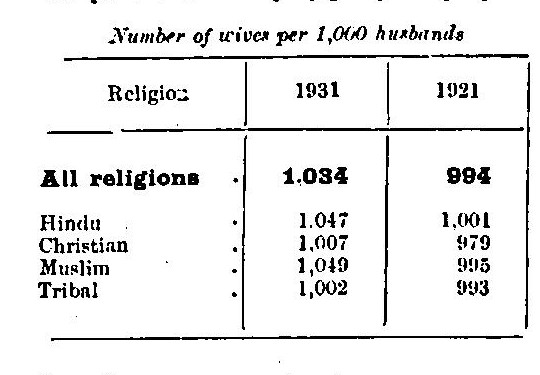
\includegraphics[width=0.5\textwidth]{wives_husbands_statistic}
\end{center}
\end{figure}

Throughout the report an attempt to
institutionalize marriage, with the State being
the body which recognizes the institution is
evident. Although the State was willing to accommodate the
existing customs, it's also willing to overthrow
the existing system of marriage altogether so that
governance becomes easy for the auxiliary bodies
maintaining the State.

In a span of 20 years post it's introduction, the
Malabar Marriage Act got only 6 marriage
registered under it, all of whom where Sir. C
Shankaran Nair's relatives
\cite{panikkar1918some}. But the effects in the
long term indicate something totally different.

\subsection{Indirect Interventions}

Another domain where the State brought about large
reforms was Education. The Colonial State had
discarded all indigenous knowledge and
incorporated Western knowledge into the curriculum
and textbooks. 

An education code in
1909-10\cite{jeffrey1987governments} laid down
instructions which made the government own the
responsibility of education of all castes and
classes of the people it governed, and a spike in
education institutions set up by missionaries. One
cannot but notice the time frame in which the
proposed reforms based on western culture arose -
within a decade of bringing about the educational
reforms in the area. An increase in the literate
population was noted by the Census of India, with
Travancore following up with Cochin and then
Malabar. The below table indicates the figures for
Travancore and Cochin.

\begin{figure}[!ht]
    \begin{center}
        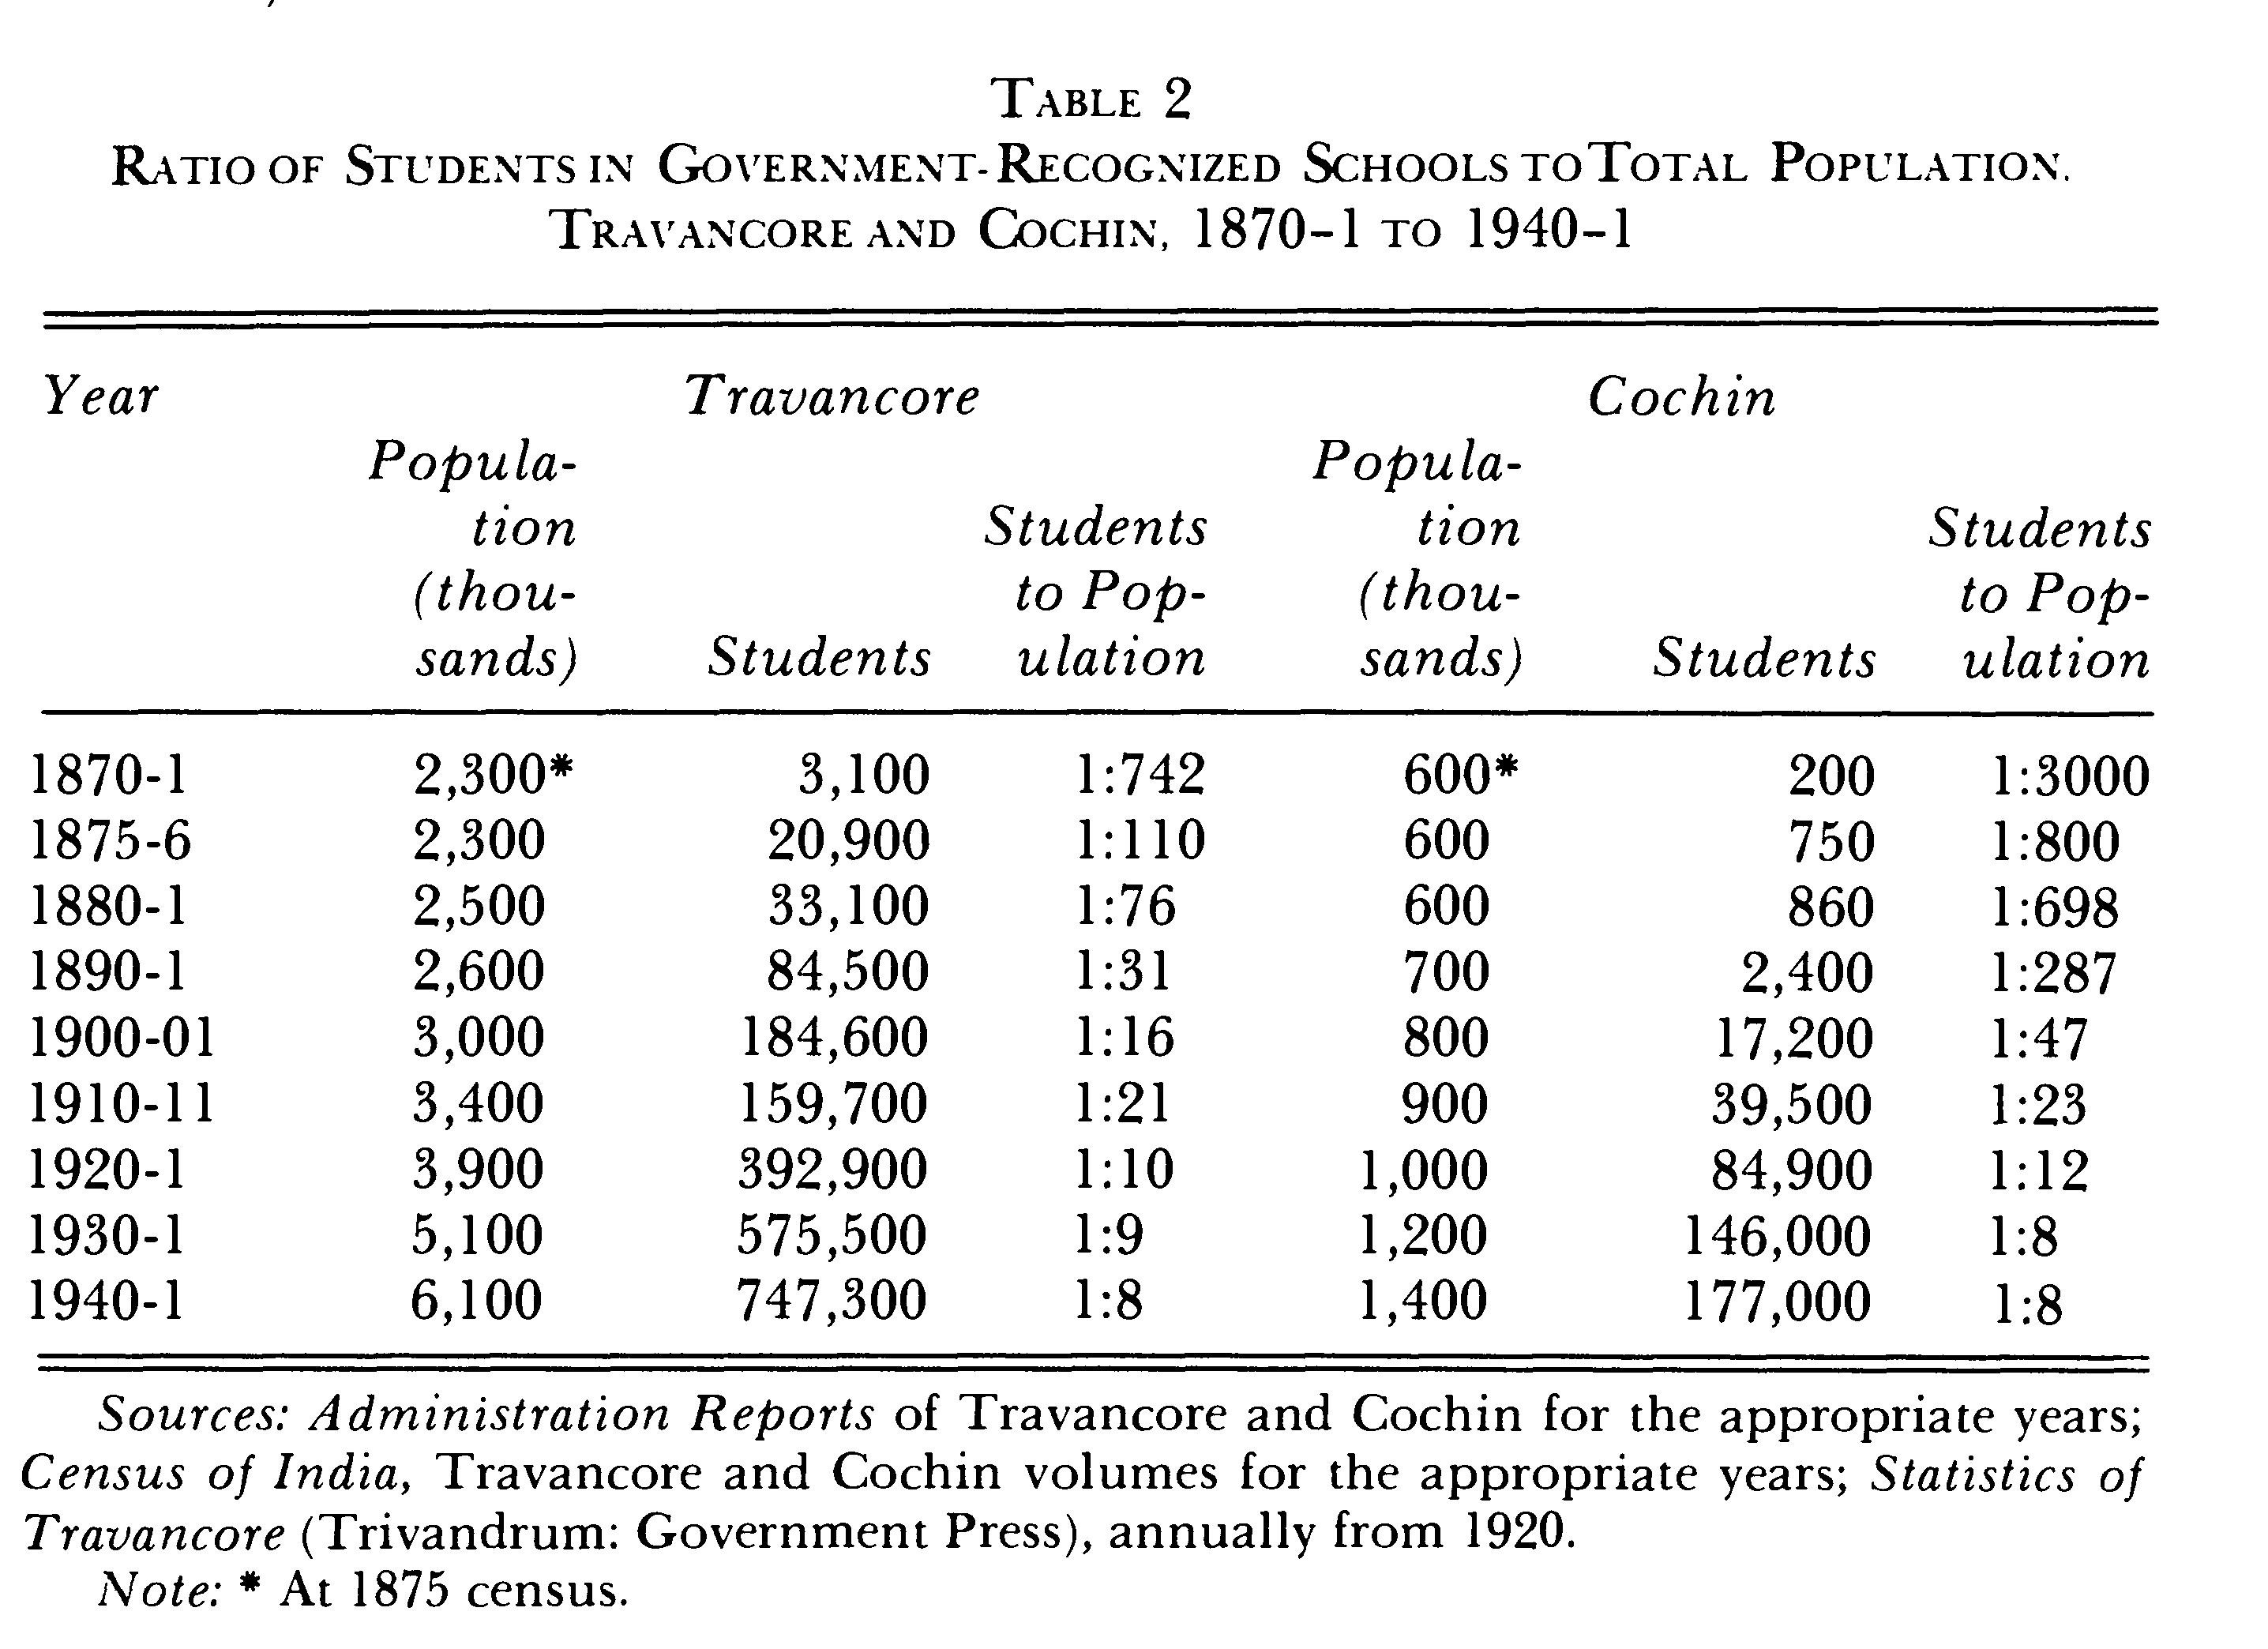
\includegraphics[width=0.8\textwidth]{education_table}
        \caption{Taken from \cite{jeffrey1987governments}}
    \end{center}
\end{figure}

Commenting on whether the legislation is expedient
or not, the Commission believed that the educated
officers who were British employed will embrace
the new legal institution of marriage, and with
them being a newly created aristocracy after the
existent Nayars and Namboodiris, the population
would follow. It is also noted that
\cite[74]{menon1894report} the educated Malayali
will keep begging for legalization of marriage.
The inevitability of the system being unworkable
with advance of education is also noted
\cite[61]{menon1894report}.

An educated witness, Mr. Rosario interviewed by
the Malabar Marriage Commission had asked around
population of North Malabar to ascertain ``there
is a growing tendency among the educated to get
the \emph{Marumakkathayam} law changed in its
entirety'' \cite[59]{menon1894report}. Commission
also argues that ``though the minority that desires
legislation is small, it is a growing and an
educated minority, and every year will add to its
strength and influence``
\cite[60]{menon1894report}.

Additionally, increased conversions from the lower
castes to Christianity and increased the cultural
mixing and led to a cultural homogenisation in
certain practices. The one-man one-woman concept
from Christianity was adopted by most of the
people in the area, following the legislations,
while the Christians to date follow
\emph{thaalikettu} as a practice, which is a Nayar
custom\cite[14]{menon1894report} wherein the
bridegroom ties a string on the bride's neck
sealing the contract of marriage.

\section{Conclusions}

Over the course of this paper, we see instances of
how the State compromised to accommodate the
customs and practices of the governed and how it
enforced its will on the people through direct and
indirect means. It is of no doubt that due to the
strong link to property succession and stability,
marriage and inheritance laws are of concern to
the State.

The State reveals itself as a social organism, which
sustains itself through its administrative bodies.
British who governed the State shouldn't have been
necessarily concerned with bringing about the
reforms, but the fact that they did, and spend
resources and time on something like this
highlights how the State would function to sustain
itself.

The people who were affected by the system had
turned towards the State for help. This is quite
indicative of the power State had over religious
customs prevalent in the area - when justice was
denied at the religious institutions, people
immediately believed that the State could bring
about justice. And the State responded positively,
had it not - it would've lost its monopoly over
the legitimized use of force in the territory.
Unwritten, unrecognised laws would've been
governing the people using which the State cannot
deliver justice. Fear of a backlash is what set
the State to instate a commission which would take
a proper statistical sample to determine the
sentiment of the masses. While dissecting the
commissions operations, we observe how
accommodation and compromises were happening at
both sides, the ones who were ruling and the
ruled.

Further, we take a look at how the State, through
indirect means like education and spread of
information prepares the people to change into a
proven stable system. The Commission had foreseen
the inevitability of the death of the
\emph{Marumakkathayam} system, which is exactly
what unrolled in the years following. It can be
concluded that education with content primarily
from the West led to a sense of shame or disgust
for the next generations and in one or two
generations even awareness of existence of
polyandry or disregard for chastity of the
\emph{Marumakkathayam} has ceased to exist. 

Angst among the colonial authorities to
\emph{Marumakkathayam} had surfaced several times
\cite{menon1894report}. The colonial sentiment
towards the systems, which were negative have
largely influenced the path taken by the reforms.
This is an effect of formalizing the succession
and marriages incorporating it in the law and the
slow brainwashing to view polyandry as evil and
chastity as a virtue.  The State couldn't have
pulled it off had the people been content with the
existing system, so one can argue that the State
used the bad influences in the social structure to
bring about the changes it desired.

\printbibliography 
\end{document}
